\chapter{PRESENTATION OF RESULTS}
\label{ch:results}

\section{Analysis of Findings}
\label{sec:analysisfindings}

All results in this chapter use the 45-case development reference described in Section~\ref{sec:analysis}. The tables are generated directly from the recomputed results file. They describe how the model behaves relative to two AI-assisted reviewers who agree with each other. They do not establish how accurate the model is.

\subsection{Overall picture}

Figure~\ref{fig:headline} summarises Table~\ref{tab:headline}. The validated v3 system and the bracket-corrected v4 system reach the same 9 of 45. The raw v4 answers are less accurate than the raw v3 answers, and on this sample the confidence intervals of all model variants overlap widely.

\begin{figure}[H]
\centering
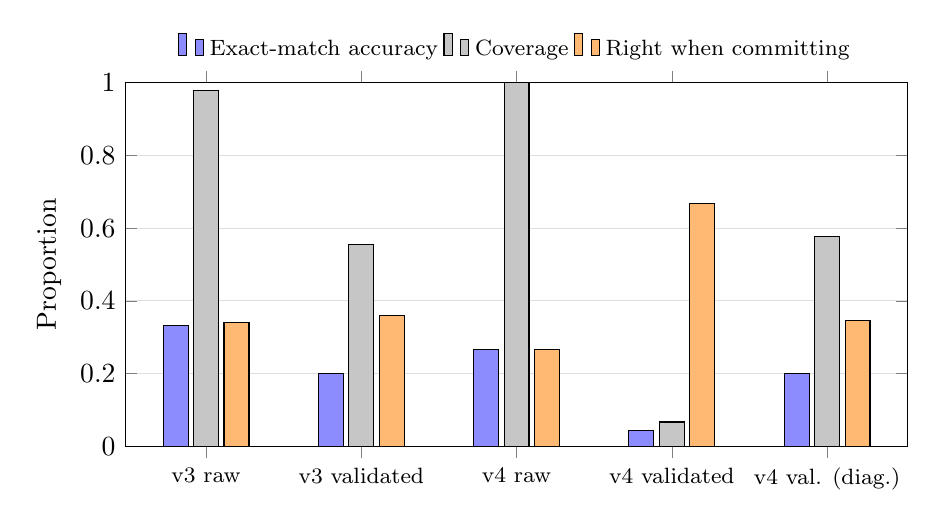
\begin{tikzpicture}
\begin{axis}[
    ybar, bar width=9pt, width=0.95\textwidth, height=6.2cm,
    ymin=0, ymax=1, ylabel={Proportion},
    symbolic x coords={v3 raw, v3 validated, v4 raw, v4 validated, v4 val. (diag.)},
    xtick=data, x tick label style={font=\footnotesize},
    legend style={at={(0.5,1.03)}, anchor=south, legend columns=3, font=\footnotesize, draw=none},
    ymajorgrids, grid style={gray!25},
    enlarge x limits=0.13]
\addplot[fill=blue!45] coordinates {(v3 raw,0.333) (v3 validated,0.2) (v4 raw,0.267) (v4 validated,0.044) (v4 val. (diag.),0.2)};
\addplot[fill=gray!45] coordinates {(v3 raw,0.978) (v3 validated,0.556) (v4 raw,1.0) (v4 validated,0.067) (v4 val. (diag.),0.578)};
\addplot[fill=orange!55] coordinates {(v3 raw,0.341) (v3 validated,0.36) (v4 raw,0.267) (v4 validated,0.667) (v4 val. (diag.),0.346)};
\legend{Exact-match accuracy, Coverage, Right when committing}
\end{axis}
\end{tikzpicture}
\caption[{Accuracy, coverage and conditional accuracy on the 45 development cases}]{Accuracy, coverage and conditional accuracy on the 45 development cases (values in Table~\ref{tab:headline}). ``v4 val.\ (diag.)'' is the diagnostic with citation brackets removed. The 0.67 of v4 validated rests on only 3 commitments.}
\label{fig:headline}
\end{figure}

\subsection{Confusion between equivalence, hierarchy, overlap and relatedness}

Table~\ref{tab:confraw} is the confusion matrix of the v3 raw answers. Three patterns stand out.

\begin{table}[H]
\centering
\small
\resizebox{\textwidth}{!}{\begin{tabular}{@{}lccccccccc@{}}
\toprule
\textbf{Reference} $\downarrow$ / \textbf{v3 raw} $\rightarrow$ & \rotatebox{70}{\SC} & \rotatebox{70}{\PA} & \rotatebox{70}{\CH} & \rotatebox{70}{\PO} & \rotatebox{70}{\RE} & \rotatebox{70}{\UN} & \rotatebox{70}{\AM} & \rotatebox{70}{\IE} & \textbf{Total} \\
\midrule
\SC & \cellcolor{green!25}\textbf{8} & \textcolor{gray!60}{0} & \textcolor{gray!60}{0} & \textcolor{gray!60}{0} & \textcolor{gray!60}{0} & \cellcolor{red!22}2 & \textcolor{gray!60}{0} & \textcolor{gray!60}{0} & 10 \\
\PA & \textcolor{gray!60}{0} & \textcolor{gray!60}{0} & \textcolor{gray!60}{0} & \textcolor{gray!60}{0} & \cellcolor{red!34}4 & \textcolor{gray!60}{0} & \textcolor{gray!60}{0} & \textcolor{gray!60}{0} & 4 \\
\CH & \cellcolor{red!50}7 & \textcolor{gray!60}{0} & \textcolor{gray!60}{0} & \cellcolor{red!16}1 & \cellcolor{red!28}3 & \cellcolor{red!16}1 & \textcolor{gray!60}{0} & \textcolor{gray!60}{0} & 12 \\
\PO & \cellcolor{red!40}5 & \textcolor{gray!60}{0} & \textcolor{gray!60}{0} & \textcolor{gray!60}{0} & \cellcolor{red!16}1 & \cellcolor{red!16}1 & \textcolor{gray!60}{0} & \textcolor{gray!60}{0} & 7 \\
\RE & \cellcolor{red!16}1 & \textcolor{gray!60}{0} & \textcolor{gray!60}{0} & \textcolor{gray!60}{0} & \cellcolor{green!25}\textbf{1} & \textcolor{gray!60}{0} & \textcolor{gray!60}{0} & \textcolor{gray!60}{0} & 2 \\
\UN & \textcolor{gray!60}{0} & \textcolor{gray!60}{0} & \textcolor{gray!60}{0} & \textcolor{gray!60}{0} & \textcolor{gray!60}{0} & \cellcolor{green!25}\textbf{6} & \textcolor{gray!60}{0} & \cellcolor{red!16}1 & 7 \\
\IE & \textcolor{gray!60}{0} & \textcolor{gray!60}{0} & \textcolor{gray!60}{0} & \textcolor{gray!60}{0} & \textcolor{gray!60}{0} & \cellcolor{red!28}3 & \textcolor{gray!60}{0} & \textcolor{gray!60}{0} & 3 \\
\midrule
\textbf{Predicted} & 21 & 0 & 0 & 1 & 9 & 13 & 0 & 1 & 45 \\
\bottomrule
\end{tabular}
}
\caption[{Confusion matrix, v3 raw answers (45 cases)}]{Confusion matrix, v3 raw answers against the R02/R03 agreement (45 cases). Diagonal in green, errors shaded by count.}
\label{tab:confraw}
\end{table}

\paragraph{Hierarchy is not recognised.} The \PA{} and \CH{} columns are empty: the model never asserted a hierarchical relation, although the reviewers gave one in 16 cases (12 \CH, 4 \PA). Narrower concepts were mostly called the same as their broader concept, and broader concepts were all called merely related.

\paragraph{\SC{} absorbs neighbouring classes.} Of the 21 raw \SC{} answers, 8 match the reference. The other 13 are 7 narrower concepts, 5 partial overlaps and 1 related pair. The model treats ``closely related'' as ``the same''.

\paragraph{Insufficient context is not recognised.} In the three cases where both reviewers judged that the context does not decide the relation, all short forms (``re'' twice, ``it''), the model answered \UN. That is a definite claim of a different sense rather than an admission that the text is insufficient.

Table~\ref{tab:errorcases} lists the three most frequent error categories, case by case. Because each case has exactly one reference and one raw answer, the categories do not overlap: together they account for 16 of the 30 raw errors. The remaining 14 errors are spread thinly: \CH~$\rightarrow$~\RE{} (3), \IE~$\rightarrow$~\UN{} (3), \SC~$\rightarrow$~\UN{} (2), and six single cases.

\begin{table}[H]
\centering
\small
\renewcommand{\arraystretch}{1.1}
\begin{tabularx}{\textwidth}{@{}p{1.5cm}X X@{}}
\toprule
\textbf{Case} & \textbf{Concept A (source)} & \textbf{Concept B (ESCO concept or topic)} \\
\midrule
\multicolumn{3}{@{}l}{\textbf{Narrower concept called same (\CH~$\rightarrow$~\SC): 7 cases}} \\
bm1-010 & MS Excel & use spreadsheets software \\
bm1-020 & MS Excel & use spreadsheets software \\
bm1-037 & cloud computing & cloud technologies \\
bm1-059 & google docs & office software \\
bm1-080 & Database Management Systems & database \\
bm1-084 & Convolutional Neural Network: The Convolution Operation & deep learning \\
bm1-086 & Python for Data Science & Python (computer programming) \\
\addlinespace
\multicolumn{3}{@{}l}{\textbf{Partial overlap called same (\PO~$\rightarrow$~\SC): 5 cases}} \\
bm1-002 & quality systems & quality control systems \\
bm1-031 & data privacy & data protection \\
bm1-052 & ict & computer technology \\
bm1-058 & conflict resolution & conflict management \\
bm1-060 & collaborate with colleagues & liaise with colleagues \\
\addlinespace
\multicolumn{3}{@{}l}{\textbf{Broader concept called related (\PA~$\rightarrow$~\RE): 4 cases}} \\
bm1-034 & financial planning & financial forecasting \\
bm1-053 & quality management & quality assurance procedures \\
bm1-063 & vector & vector line integrals \\
bm1-070 & Equations & equations solvable for y \\
\addlinespace
\bottomrule
\end{tabularx}

\caption[{The three most frequent error categories of the v3 raw answers}]{The three most frequent error categories of the v3 raw answers. The counts 7, 5 and 4 reproduce the figures reported during development.}
\label{tab:errorcases}
\end{table}

Two of the narrower-as-same cases appear twice under different case identifiers (``MS Excel'' in bm1-010 and bm1-020). The benchmark contains separate candidates for the same surface pair in different postings, so the 7 cases correspond to 6 distinct term pairs.

\subsection{Per-class behaviour}

Table~\ref{tab:prf} gives per-class precision, recall and F1. With 2 to 12 reference cases per class these values are very imprecise and are reported only to show the pattern. The pattern is consistent with the confusion matrix. \UN{} and \SC{} have the highest recall. \PA, \CH{} and \PO{} have zero recall. Validation lowers recall for \SC{} (0.80 to 0.30) without raising precision much (0.38 to 0.43), and moves 18 answers to \IE, none of which matches an \IE{} reference.

\begin{table}[H]
\centering
\small
\resizebox{\textwidth}{!}{\begin{tabular}{@{}lr|rrrr|rrrr@{}}
\toprule
 & & \multicolumn{4}{c|}{\textbf{v3 raw}} & \multicolumn{4}{c}{\textbf{v3 validated}} \\
\textbf{Class} & \textbf{Ref.} & \textbf{Pred.} & \textbf{P} & \textbf{R} & \textbf{F1} & \textbf{Pred.} & \textbf{P} & \textbf{R} & \textbf{F1} \\
\midrule
\SC & 10 & 21 & 0.38 & 0.80 & 0.52 & 7 & 0.43 & 0.30 & 0.35 \\
\PA & 4 & 0 & -- & 0.00 & -- & 0 & -- & 0.00 & -- \\
\CH & 12 & 0 & -- & 0.00 & -- & 0 & -- & 0.00 & -- \\
\PO & 7 & 1 & 0.00 & 0.00 & 0.00 & 1 & 0.00 & 0.00 & 0.00 \\
\RE & 2 & 9 & 0.11 & 0.50 & 0.18 & 5 & 0.20 & 0.50 & 0.29 \\
\UN & 7 & 13 & 0.46 & 0.86 & 0.60 & 12 & 0.42 & 0.71 & 0.53 \\
\AM & 0 & 0 & -- & -- & -- & 2 & 0.00 & -- & -- \\
\IE & 3 & 1 & 0.00 & 0.00 & 0.00 & 18 & 0.00 & 0.00 & 0.00 \\
\midrule
Macro-F1 (reference classes) & \multicolumn{5}{r|}{0.18} & \multicolumn{4}{r}{0.17} \\
\bottomrule
\end{tabular}
}
\caption[{Per-class precision, recall and F1, v3 raw and validated answers}]{Per-class precision (P), recall (R) and F1 for v3 raw and validated answers. ``--'': undefined because the class was never predicted, or never in the reference. Macro-F1 averages over the 7 classes present in the reference, counting undefined F1 as 0.}
\label{tab:prf}
\end{table}

For orientation only, and not as an evaluation (the gate applies to independent gold, which does not exist): among the validated system's 7 \SC{} commitments, 4 differ from the reviewers' answer (2 \PO, 1 \CH, 1 \RE). Gate v3 allows at most one false \SC.

\subsection{Effect of the v4 prompt}

Table~\ref{tab:confv4} shows the raw v4 answers. The ordered decision procedure reduced \SC{} answers from 21 to 6, and the model began to use \PA. But the errors moved instead of disappearing:
\begin{itemize}
    \item 6 narrower concepts were called \RE;
    \item 4 narrower concepts were called \PA, a reversal of direction. The narrower ``cloud computing'' was called broader than ``cloud technologies'' (bm1-037).
    \item 4 partial overlaps were called \RE.
\end{itemize}
Raw accuracy fell from 15 to 12. With the citation defect neutralised, the validated score equalled v3's 9. This is consistent with the project's conclusion that breadth and direction judgements are a limit of the 7B model rather than of the wording alone. The evidence for that conclusion is limited to one prompt revision, one model and 45 cases.

\begin{table}[H]
\centering
\small
\resizebox{\textwidth}{!}{\begin{tabular}{@{}lccccccccc@{}}
\toprule
\textbf{Reference} $\downarrow$ / \textbf{v4 raw} $\rightarrow$ & \rotatebox{70}{\SC} & \rotatebox{70}{\PA} & \rotatebox{70}{\CH} & \rotatebox{70}{\PO} & \rotatebox{70}{\RE} & \rotatebox{70}{\UN} & \rotatebox{70}{\AM} & \rotatebox{70}{\IE} & \textbf{Total} \\
\midrule
\SC & \cellcolor{green!25}\textbf{4} & \cellcolor{red!22}2 & \textcolor{gray!60}{0} & \textcolor{gray!60}{0} & \cellcolor{red!22}2 & \cellcolor{red!22}2 & \textcolor{gray!60}{0} & \textcolor{gray!60}{0} & 10 \\
\PA & \textcolor{gray!60}{0} & \textcolor{gray!60}{0} & \textcolor{gray!60}{0} & \cellcolor{red!22}2 & \cellcolor{red!22}2 & \textcolor{gray!60}{0} & \textcolor{gray!60}{0} & \textcolor{gray!60}{0} & 4 \\
\CH & \textcolor{gray!60}{0} & \cellcolor{red!34}4 & \textcolor{gray!60}{0} & \textcolor{gray!60}{0} & \cellcolor{red!46}6 & \cellcolor{red!22}2 & \textcolor{gray!60}{0} & \textcolor{gray!60}{0} & 12 \\
\PO & \cellcolor{red!16}1 & \cellcolor{red!16}1 & \textcolor{gray!60}{0} & \textcolor{gray!60}{0} & \cellcolor{red!34}4 & \cellcolor{red!16}1 & \textcolor{gray!60}{0} & \textcolor{gray!60}{0} & 7 \\
\RE & \cellcolor{red!16}1 & \textcolor{gray!60}{0} & \textcolor{gray!60}{0} & \textcolor{gray!60}{0} & \cellcolor{green!25}\textbf{1} & \textcolor{gray!60}{0} & \textcolor{gray!60}{0} & \textcolor{gray!60}{0} & 2 \\
\UN & \textcolor{gray!60}{0} & \textcolor{gray!60}{0} & \textcolor{gray!60}{0} & \textcolor{gray!60}{0} & \textcolor{gray!60}{0} & \cellcolor{green!25}\textbf{7} & \textcolor{gray!60}{0} & \textcolor{gray!60}{0} & 7 \\
\IE & \textcolor{gray!60}{0} & \textcolor{gray!60}{0} & \textcolor{gray!60}{0} & \textcolor{gray!60}{0} & \textcolor{gray!60}{0} & \cellcolor{red!28}3 & \textcolor{gray!60}{0} & \textcolor{gray!60}{0} & 3 \\
\midrule
\textbf{Predicted} & 6 & 7 & 0 & 2 & 15 & 15 & 0 & 0 & 45 \\
\bottomrule
\end{tabular}
}
\caption[{Confusion matrix, v4 raw answers (45 cases)}]{Confusion matrix, v4 raw answers (45 cases).}
\label{tab:confv4}
\end{table}

\subsection{Results by case kind}

Table~\ref{tab:bykind} breaks the results down by case kind. All six correct answers that validation withheld are alias cases (9 raw to 3 validated). Four of them were withheld only for a missing concept-side citation. The numbers per kind are too small for comparison between kinds.

\begin{table}[H]
\centering
\small
\begin{tabular}{@{}lrrrr@{}}
\toprule
\textbf{Case kind} & \textbf{Cases} & \textbf{v3 raw} & \textbf{v3 validated} & \textbf{v4 raw} \\
\midrule
\inputrows{generated/by_kind.tex}
\bottomrule
\end{tabular}
\caption[{Correct answers by case kind (45 development cases)}]{Correct answers by case kind (45 development cases).}
\label{tab:bykind}
\end{table}

\subsection{Reviewer agreement}

Table~\ref{tab:pairwise} gives Cohen's $\kappa$ and the number of agreements for every pair of the five reviewer records over the 48 cases. R02 and R03 agree far more closely ($\kappa=0.92$, 45 of 48) than any other pair ($\kappa$ between 0.56 and 0.76). This is consistent with their shared process of consulting an AI assistant first, but does not by itself establish it. The three R02/R03 disagreements concern ``Information Management'' versus ``knowledge management'' (\RE{} vs \PO) and the abbreviation ``ml'' in two cases, where R02 judged the context ambiguous.

\begin{table}[H]
\centering
\small
\begin{tabular}{@{}lccccc@{}}
\toprule
 & \textbf{R01} & \textbf{R02} & \textbf{R03} & \textbf{R04} & \textbf{R05} \\
\midrule
R01 & -- & 0.66 (34) & 0.64 (33) & 0.56 (30) & 0.59 (31) \\
R02 & 0.66 (34) & -- & 0.92 (45) & 0.63 (33) & 0.75 (38) \\
R03 & 0.64 (33) & 0.92 (45) & -- & 0.65 (34) & 0.73 (37) \\
R04 & 0.56 (30) & 0.63 (33) & 0.65 (34) & -- & 0.76 (38) \\
R05 & 0.59 (31) & 0.75 (38) & 0.73 (37) & 0.76 (38) & -- \\
\bottomrule
\end{tabular}

\caption[{Pairwise Cohen's $\kappa$ between the five reviewer records}]{Pairwise Cohen's $\kappa$ (number of agreements out of 48) between the five reviewer records. None of the records is an independent label set (Table~\ref{tab:reviewers}).}
\label{tab:pairwise}
\end{table}

The benchmark's development labels, written by an AI assistant, match the R02/R03 consensus in only 25 of the 45 cases. This supports the project's rule that development labels are for stratification and diagnostics only. It also shows that even two AI-informed sources can differ widely on these distinctions.

\subsection{Case-level record}

Table~\ref{tab:percase} lists every scored case so that each figure in this chapter can be traced. A bold label marks agreement with the reference.

{\small
\setlength{\tabcolsep}{4pt}
\begin{longtable}{@{}p{1.45cm}p{3.9cm}p{3.45cm}cccc@{}}
\caption[{All 45 development cases: reference and system answers}]{All 45 development cases: reference (R02 = R03) and system answers. SC = \SC, PA = \PA, CH = \CH, PO = \PO, RE = \RE, UN = \UN, AM = \AM, IE = \IE.}\label{tab:percase}\\
\toprule
\textbf{Case} & \textbf{Concept A} & \textbf{Concept B} & \textbf{Ref.} & \textbf{v3 raw} & \textbf{v3 val.} & \textbf{v4 raw} \\
\midrule
\endfirsthead
\toprule
\textbf{Case} & \textbf{Concept A} & \textbf{Concept B} & \textbf{Ref.} & \textbf{v3 raw} & \textbf{v3 val.} & \textbf{v4 raw} \\
\midrule
\endhead
\bottomrule
\endfoot
\inputrows{generated/per_case.tex}
\end{longtable}
}

\section{Comparison with Existing Work}
\label{sec:comparison}

No published study evaluates the same task on the same data, so a numerical comparison would be misleading. Table~\ref{tab:comparison} instead sets out how the related work differs from this project in task, data, method and metric. It identifies what each body of work contributes and what it does not settle for this project. No superiority is claimed in either direction.

\begin{table}[H]
\centering
\scriptsize
\renewcommand{\arraystretch}{1.25}
\begin{tabularx}{\textwidth}{@{}p{2.6cm}XXX@{}}
\toprule
\textbf{Work} & \textbf{Task and data} & \textbf{Method and metric} & \textbf{Difference from this project} \\
\midrule
STS pilot~\cite{agirre2012} & Graded similarity of sentence pairs & Human similarity scores; correlation with system scores & Scalar similarity, no relation type or direction; sentences, not terms with taxonomy context \\
Sentence-BERT~\cite{reimers2019} & Sentence embeddings for similarity search & Siamese fine-tuning; cosine similarity & Provides closeness, not the distinctions between \SC, \PA, \CH, \PO{} and \RE; the project uses TF-IDF and does not run an embedding model by default \\
Ontology matching~\cite{euzenat2013} & Correspondences between two ontologies & Typed correspondences (equivalence, subsumption, disjointness) & Closest in task; here one side is free text from postings and syllabi, with an explicit abstention option \\
Hierarchical classification~\cite{silla2011} & Assigning items to classes in a hierarchy & Hierarchy-aware evaluation & The project's labels are relation types, but its gate likewise treats direction errors as severe \\
Skill extraction and matching~\cite{sun2026,rosenberger2025,gonzalezgomez2025} & Skills in job text matched to ESCO; resume--job matching; taxonomy generation & Contrastive bi-encoders; shared embedding spaces; NER and relation extraction & Extraction and retrieval at scale; this project verifies a single typed relation for pairs the rules left open \\
LLM as judge~\cite{zheng2023} & Model judges compared with human preferences on chat answers & Agreement with human judgements; bias analysis & Same concern with model judgement reliability; here the model's labels gate data analysis and are kept advisory \\
LLM-assisted annotation~\cite{gilardi2023,veselovsky2023} & Annotation by models, and model use by crowd workers & Accuracy against expert labels; detection of model use & Explains why AI-assisted reviewer answers here are not treated as independent \\
Selective classification~\cite{chow1970,geifman2017} & Classifiers that may reject & Risk--coverage trade-off & The validator is a rule-based reject option; its thresholds are not learned, and coverage is reported alongside accuracy \\
\bottomrule
\end{tabularx}
\caption[{Comparison with related work by task, data, method and metric}]{Comparison with related work by task, data, method and metric.}
\label{tab:comparison}
\end{table}

Three differences matter most. First, this project evaluates a \emph{typed, directional} relation where much related work measures \emph{similarity}, so a high similarity score elsewhere says nothing about the hierarchy errors observed here. Second, the project scores what downstream would read after a deterministic validator, and reports abstention. Most published evaluations score raw outputs. Third, the project's reference is small and AI-assisted, while the cited studies rest on larger human-labelled datasets. Until independent labels exist, the project's figures cannot be placed on the same footing as published results.
